\subsection{Publicly Available Data}
Experiments were performed on a subset of the publicly available\footnote{http://crcns.org/data-sets/hc/hc-1/} dataset described in \cite{Henze2000}.  We used the dataset d533101 that consisted of an extracellular tetrode and a single intracellular electrode.  The recording was made simultaneously on all electrodes and was set up such cell with the intracellular electrode was also recorded on the extracellular array. 

The intracellular recording is relatively noiseless and gives nearly certain firing times of the intracellular neuron.  The extracellular recording contains the spike waveforms from the intracellular neuron as well as an unknown number of additional neurons.  The data is a 4-minute recording at a 10kHz sampling rate and preprocessed with a high-pass filter at 800 Hz.

Each algorithm gives a clustering of the detected spikes.  In this dataset, we only have a partial ground truth, so we are only able to analyze whether a spike comes from the intracellular (IC) recording or not.  In these experiments, we define a detected spike to be an IC spike if the IC recording has a spike within .5ms of the detected spike.  We define the cluster with the greatest number of intracellular spikes as a the "IC cluster."  Figure \ref{hc1res} shows the performance on the intracellular cluster versus competing methods.  The single-channel experiments were all run on channel 2 (the results were nearly identitcal for all channels).  The spike detections for the offline methods were given by using a threshold at 3 times the noise standard deviation \cite{Lewicki}. (Need to do more comparisons and descriptions) and windowed at a size $P=30$ (check if $P$ matches with Vinayak notation).  The action potential window was set at 30, and PCA was used to reduce the space to $K$=3 for the experiments.  The results were very similar for $K$=2, $K$=3, and $K$=4.   There were 3742 spikes detected with the threshold, and 753 of those corresponded to the intracellular spikes.

The online algorithms were all run with weakly informative parameters (add parameters once I get vinayak's notation). The parameters were insensitive to minor changes.  Running time in unoptimized MATLAB code for 4 minutes of data was 31s was a single channel and 3 minutes for all 4 channels on a 3.2GHzIntel Core i5 machine with 6GB of memory.  We show the inferred $y_k$ fordetected spikes in the 2-PCA space in Figure \ref{pcaonlinear}.

As as been demonstrated previously (cite paninski), the waveform shape of a neuron may change over time.  The mean waveform over time for the intracellular neuron is shown in Figure \ref{evohc1}.  For the IC cluster, it is of interest to investigate the properties of the true positives, the false positives, as well as the IC spikes that are missed by the algorithm.  Errorbar plots for these groups are shown in Figure \ref{truewaveforms}; this figure demonstrates the great similarity of the true positives and the false positives, while the missed positives (spike waveforms not detected or not in the IC cluster) have high variability and a different mean shape.

To get an idea of the robustness of the algorithm, we split the data into random segments of 2minutes, and ran the algorithms on that dataset.  Add plot and information.
\section{Multi-Electrode Sensors}
In the tetrode case the spike undoubtedly appears on all channels at once.  Often, people will just concatenate the channels to process the data (eg. cites).  When the action potential will only appear on a subset of channels it is nice to allow the action potential to vary in a low-dimensional subset in each of the channels instead of a low-dimensional subset over all the channels.  This is especially important when the appropriate dictionary is not known beforehand.

We use processed data from novel NeuroNexus devices.  (Need to give a description of this).  The first device we consider is a set of 3 channels of data shown in Figure \ref{3dev}.  The neighboring electrode sites in these devices have 30 $\mu$m between electrode edges and 60 $\mu$m between electrode centers.  These devices are close enough that a locally-firing neuron could appear on multiple electrode sites (cite that paper on action potential overlap), and neighboring channels warrant joint processing.

 The top 3 clusters found in the first 10 minutes of data are shown in Figure (add in a bit).


\begin{center}
\begin{figure}
\begin{subfigure}[b]{.5\textwidth}
\centering
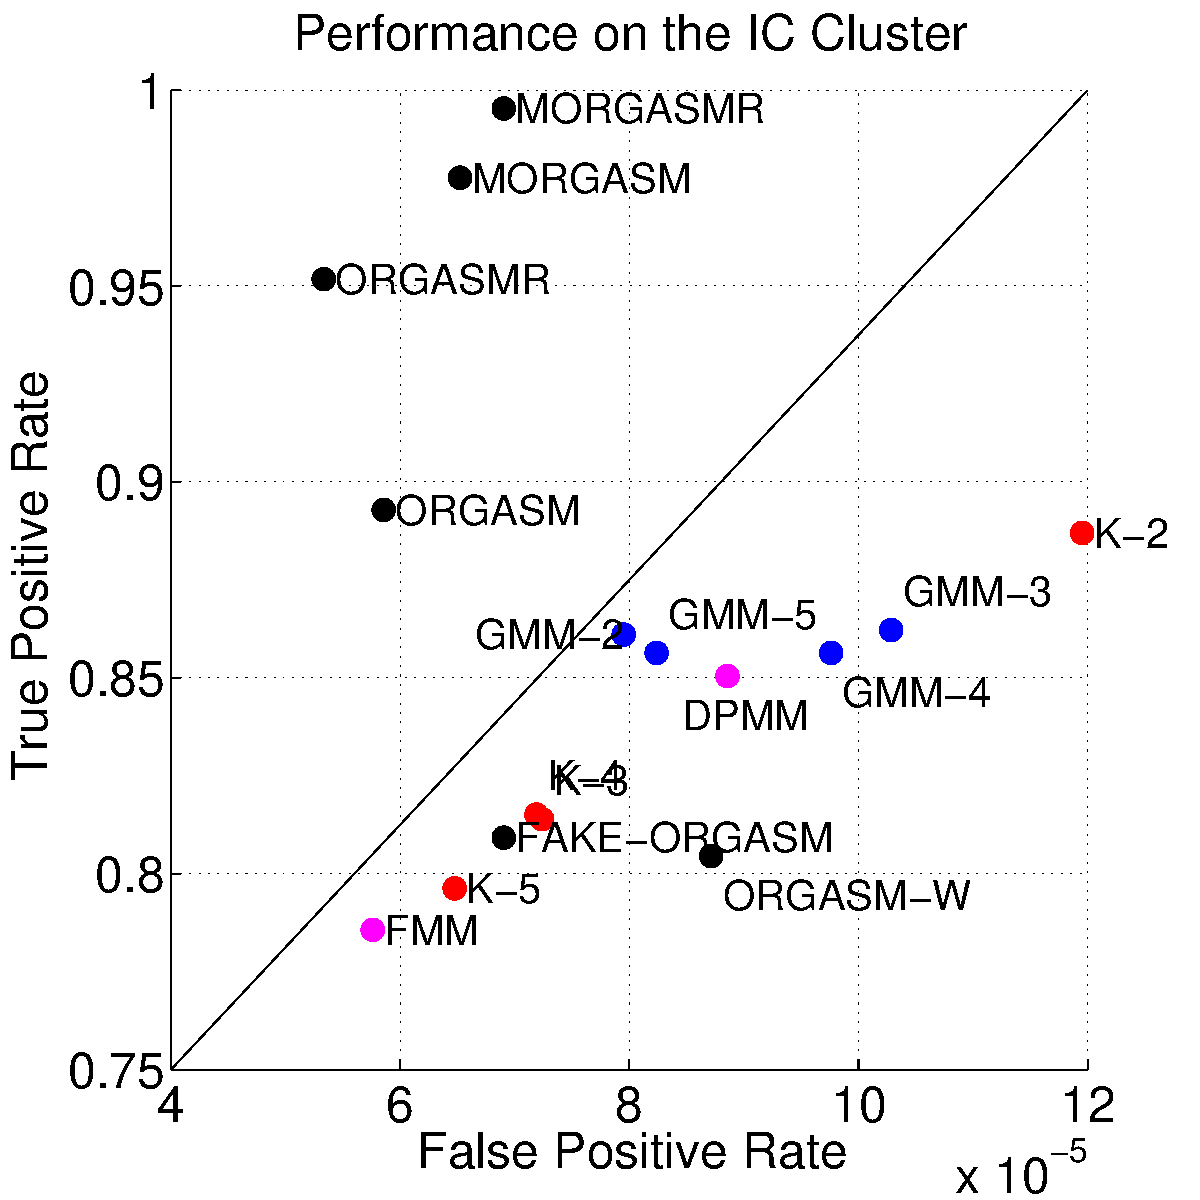
\includegraphics[width=\textwidth]{../figs/truefalsepositive}
\caption{}
\label{hc1res}
\end{subfigure}
\begin{subfigure}[b]{.5\textwidth}
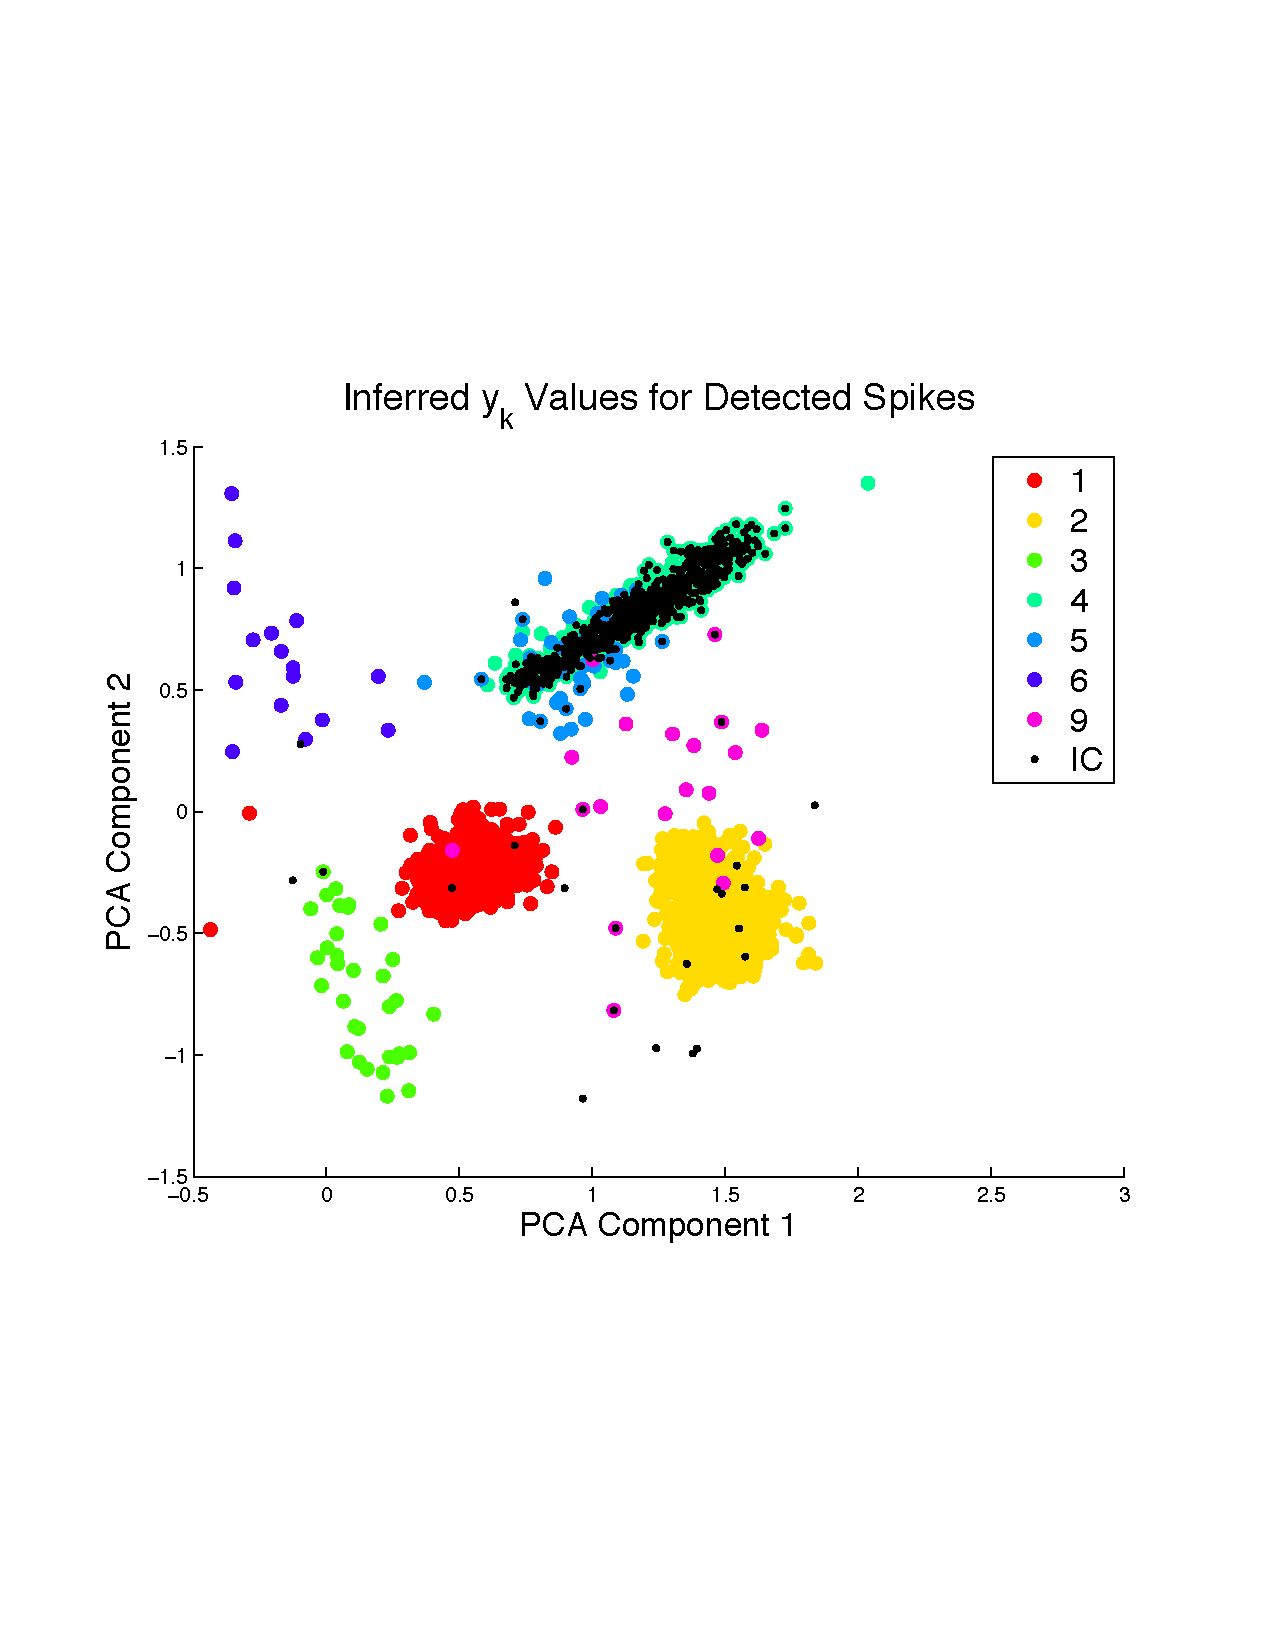
\includegraphics[width=\textwidth]{../figs/ykarreduced}
\caption{}
\label{pcaonlinear}
\end{subfigure}
\caption{Results on the d533101 dataset.  (a) This shows the number of true positives versus the number of false positives.  Our methods do better, yay! (b) Results on the d533101 dataset from the online algorithm with an AR mean}
\end{figure}
\end{center}
\begin{center}





\begin{figure}
\begin{subfigure}[b]{.5\textwidth}
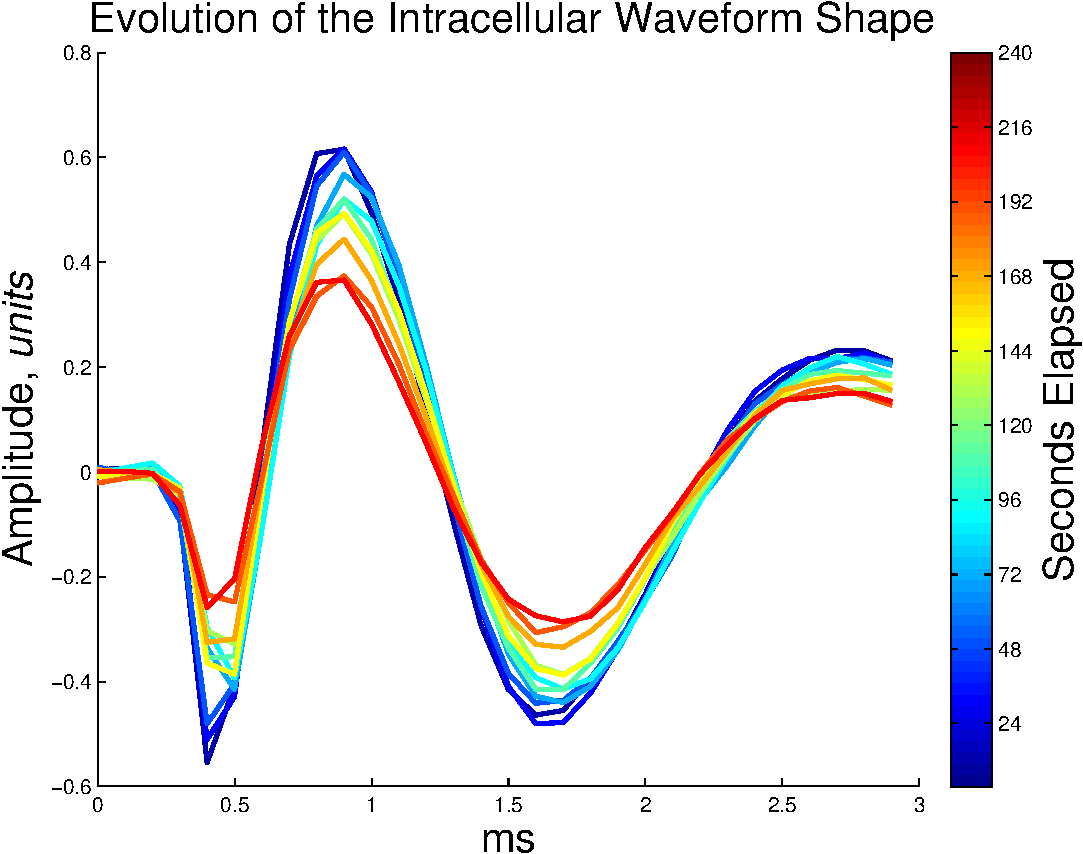
\includegraphics[width=\textwidth]{../figs/evohc1}
\caption{}
\label{evohc1}
\end{subfigure}
\begin{subfigure}[b]{.5\textwidth}
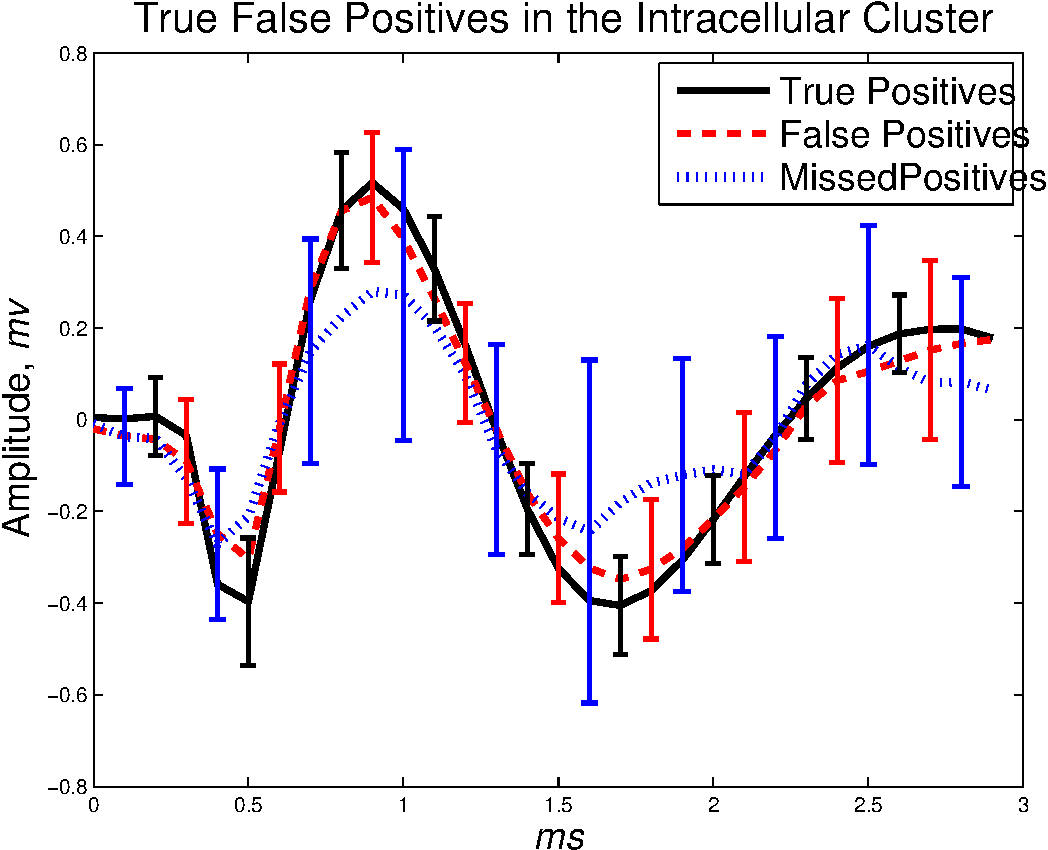
\includegraphics[width=\textwidth]{../figs/IntracellularTrueFalsePositivesv2}
\caption{}
\label{truewaveforms}
\end{subfigure}



\caption{(a) Mean IC waveforms over time.  Each colored line represents the mean of the waveform averaged over 24s and the color gives the elapsed time.  This neuron decreases in amplitude over the period of the recording. (b) Errorbar plots of the true positives and the false positives in the IC cluster.  While the false positives have slightly more variability, the mean shape for the false positives and the true positives is nearly identical.  The true misses have a significantly lower amplitude as well as high variability}
\end{figure}
\end{center}
\begin{center}
\begin{figure}
\begin{subfigure}[b]{.24\textwidth}
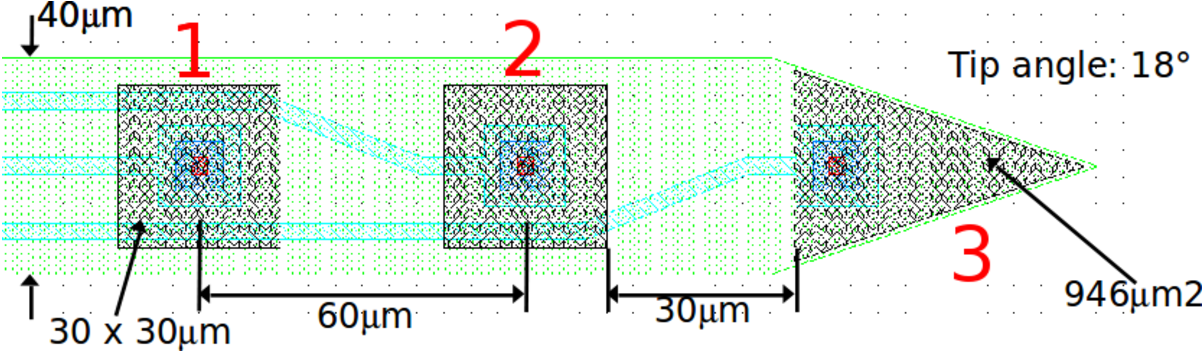
\includegraphics[width=\textwidth]{../figs/3dev}
\caption{}
\label{3dev}
\end{subfigure}
\begin{subfigure}[b]{.24\textwidth}
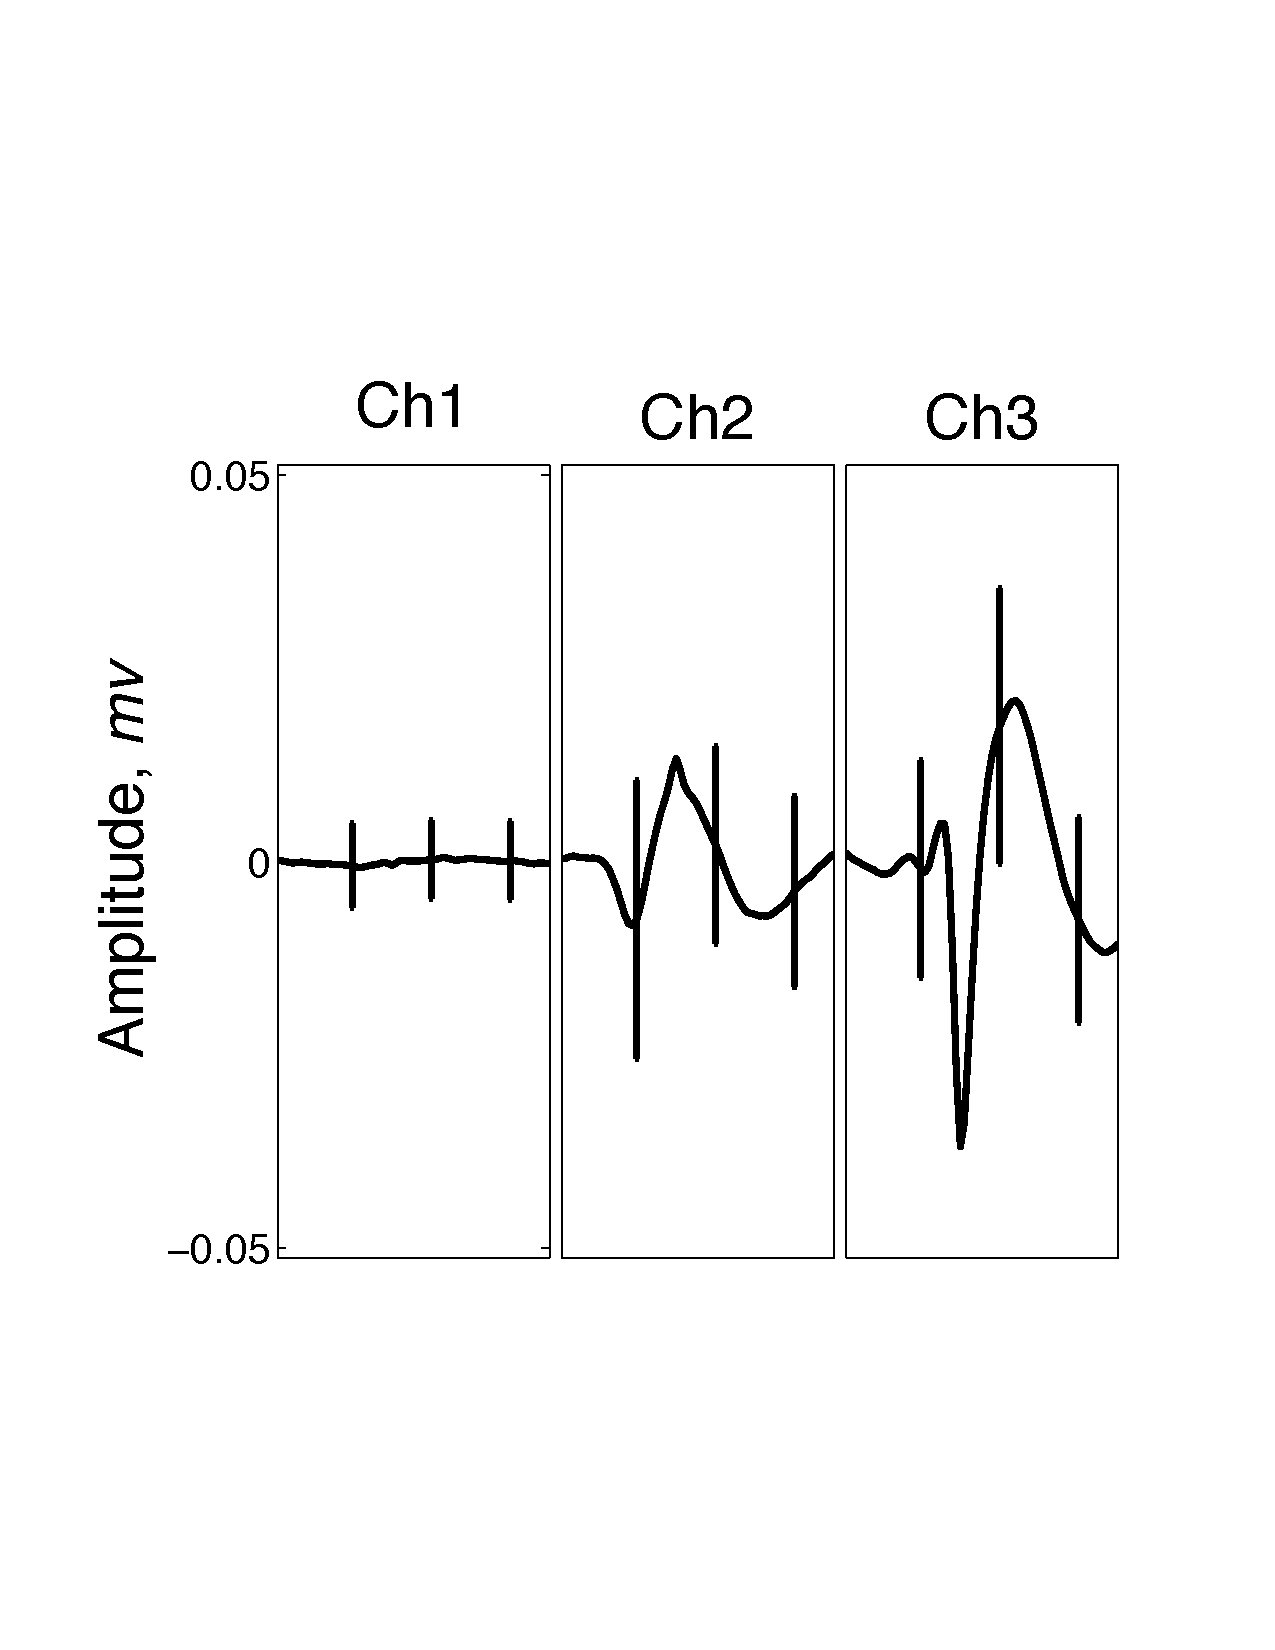
\includegraphics[width=\textwidth]{../figs/3devim/clus1}
\caption{}
\end{subfigure}
\begin{subfigure}[b]{.24\textwidth}
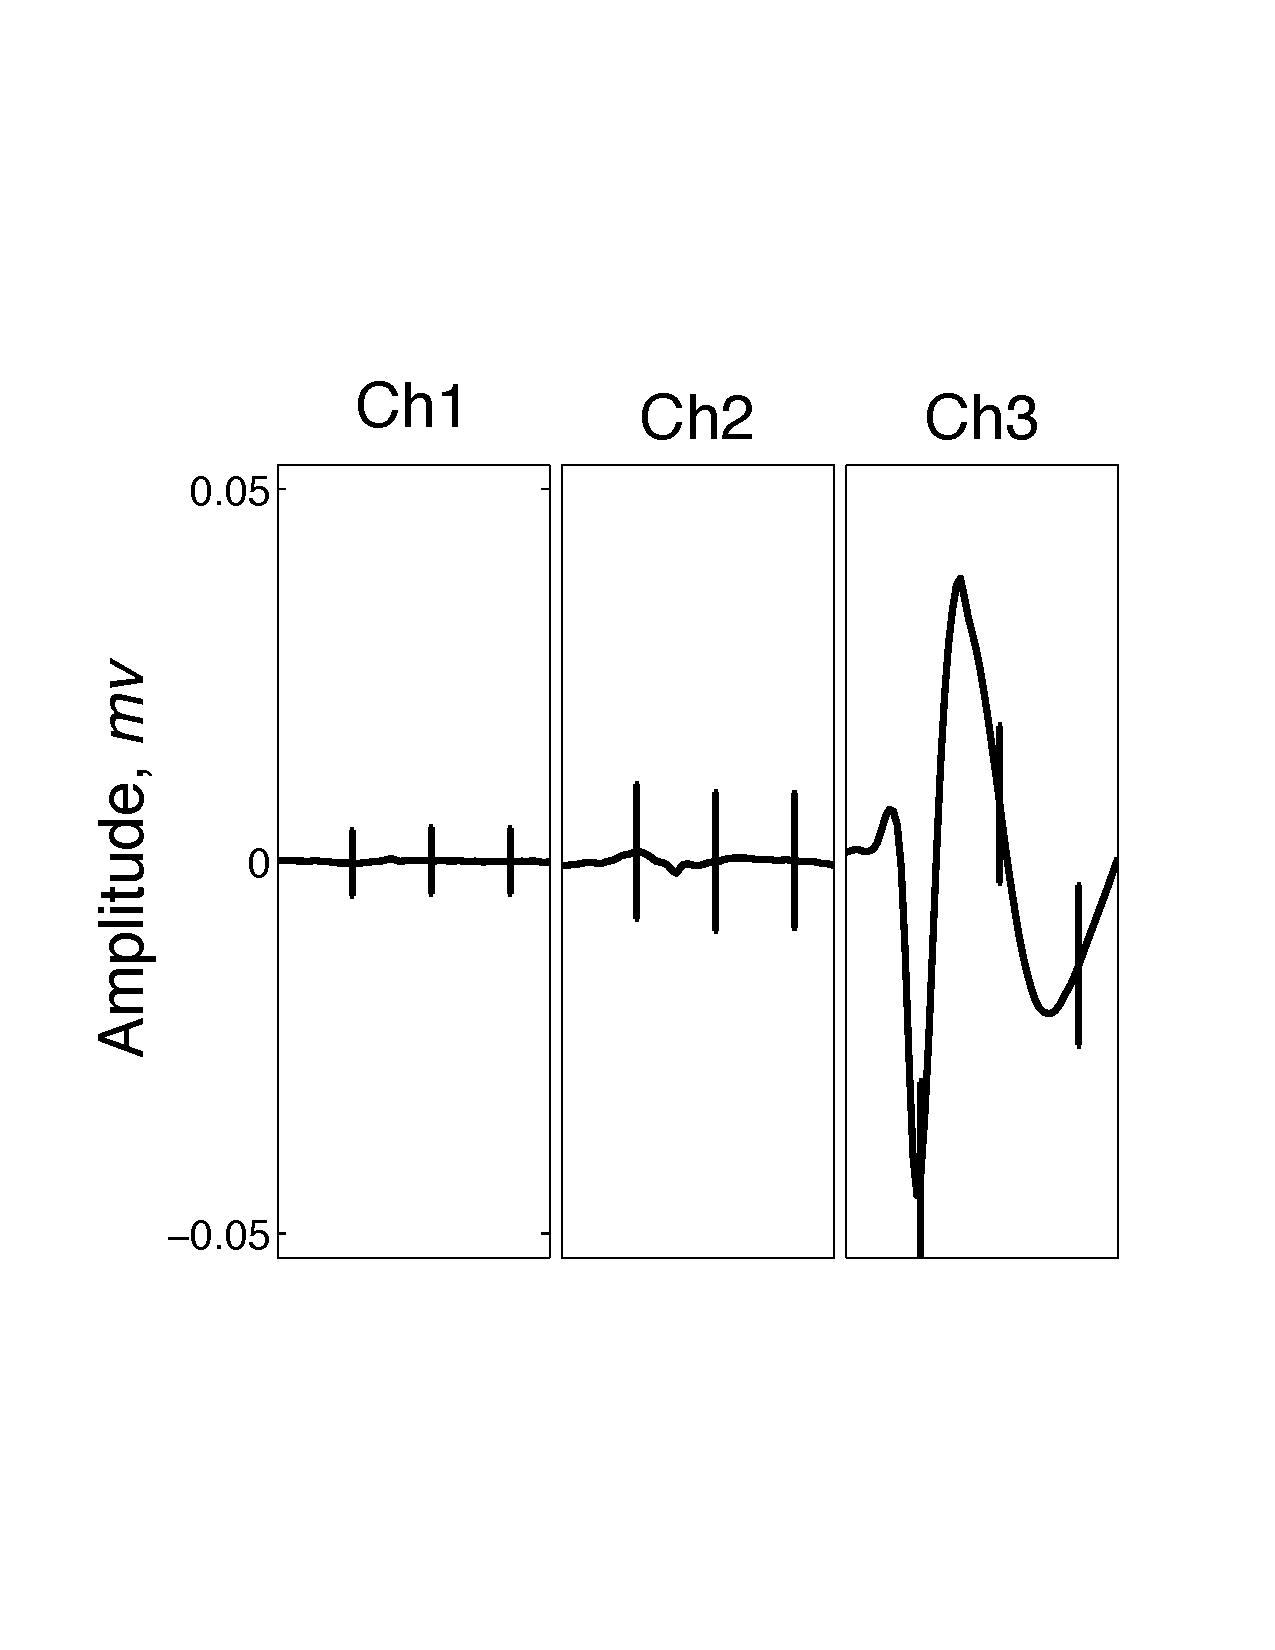
\includegraphics[width=\textwidth]{../figs/3devim/clus2}
\caption{}
\end{subfigure}
\begin{subfigure}[b]{.24\textwidth}
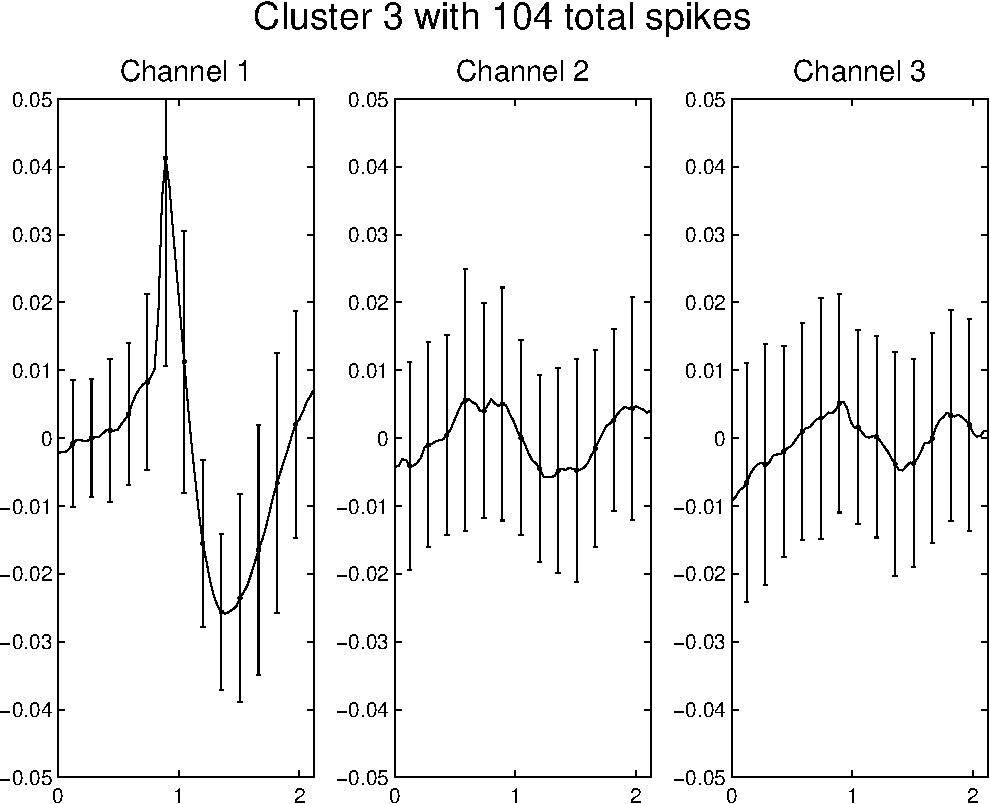
\includegraphics[width=\textwidth]{../figs/3devim/clus3}
\caption{}
\end{subfigure}
\caption{Device used. Channels in large, red numbers.}
\end{figure}
\end{center}